\documentclass[12pt, titlepage]{article}

\usepackage{fullpage}
\usepackage[round]{natbib}
\usepackage{multirow}
\usepackage{booktabs}
\usepackage{tabularx}
\usepackage{graphicx}
\usepackage{svg}
\usepackage{float}
\usepackage{hyperref}
\hypersetup{
    colorlinks,
    citecolor=blue,
    filecolor=black,
    linkcolor=red,
    urlcolor=blue
}

%% Comments

\usepackage{color}

\newif\ifcomments\commentstrue %displays comments
%\newif\ifcomments\commentsfalse %so that comments do not display

\ifcomments
\newcommand{\authornote}[3]{\textcolor{#1}{[#3 ---#2]}}
\newcommand{\todo}[1]{\textcolor{red}{[TODO: #1]}}
\else
\newcommand{\authornote}[3]{}
\newcommand{\todo}[1]{}
\fi

\newcommand{\wss}[1]{\authornote{blue}{SS}{#1}} 
\newcommand{\plt}[1]{\authornote{magenta}{TPLT}{#1}} %For explanation of the template
\newcommand{\an}[1]{\authornote{cyan}{Author}{#1}}

%% Common Parts

\newcommand{\progname}{ProgName} % PUT YOUR PROGRAM NAME HERE
\newcommand{\authname}{Team \#, Team Name
\\ Student 1 name
\\ Student 2 name
\\ Student 3 name
\\ Student 4 name} % AUTHOR NAMES                  

\usepackage{hyperref}
    \hypersetup{colorlinks=true, linkcolor=blue, citecolor=blue, filecolor=blue,
                urlcolor=blue, unicode=false}
    \urlstyle{same}
                                


\newcounter{acnum}
\newcommand{\actheacnum}{AC\theacnum}
\newcommand{\acref}[1]{AC\ref{#1}}

\newcounter{ucnum}
\newcommand{\uctheucnum}{UC\theucnum}
\newcommand{\uref}[1]{UC\ref{#1}}

\newcounter{mnum}
\newcommand{\mthemnum}{M\themnum}
\newcommand{\mref}[1]{M\ref{#1}}

\begin{document}

\title{Module Guide for \progname{}} 
\author{\authname}
\date{\today}

\maketitle

\pagenumbering{roman}

\section{Revision History}

\begin{tabularx}{\textwidth}{p{3cm}p{2cm}X}
\toprule {\bf Date} & {\bf Version} & {\bf Notes}\\
\midrule
01/17/2023 & 1.0 & Initial Draft\\
01/18/2023 & 1.1 & Small fixes\\
04/03/2023 & 1.2 & Added higher quality diagrams. Updated unlikely changes.\\
\bottomrule
\end{tabularx}

\newpage

\section{Reference Material}

This section records information for easy reference.

\subsection{Abbreviations and Acronyms}

\renewcommand{\arraystretch}{1.2}
\begin{tabular}{l l} 
  \toprule		
  \textbf{symbol} & \textbf{description}\\
  \midrule 
  AC & Anticipated Change\\
  DAG & Directed Acyclic Graph \\
  M & Module \\
  MG & Module Guide \\
  OS & Operating System \\
  R & Requirement\\
  SC & Scientific Computing \\
  SRS & Software Requirements Specification\\
  \progname & The Software Engineering Capstone Project Course at McMaster University\\
  UC & Unlikely Change \\
  \bottomrule
\end{tabular}\\

\newpage

\tableofcontents

\listoftables

\listoffigures

\newpage

\pagenumbering{arabic}

\section{Introduction}

Decomposing a system into modules is a commonly accepted approach to developing
software.  A module is a work assignment for a programmer or programming
team~\citep{ParnasEtAl1984}.  We advocate a decomposition
based on the principle of information hiding~\citep{Parnas1972a}.  This
principle supports design for change, because the ``secrets'' that each module
hides represent likely future changes.  Design for change is valuable in SC,
where modifications are frequent, especially during initial development as the
solution space is explored.  

Our design follows the rules layed out by \citet{ParnasEtAl1984}, as follows:
\begin{itemize}
\item System details that are likely to change independently should be the
  secrets of separate modules.
\item Each data structure is implemented in only one module.
\item Any other program that requires information stored in a module's data
  structures must obtain it by calling access programs belonging to that module.
\end{itemize}

After completing the first stage of the design, the Software Requirements
Specification (SRS), the Module Guide (MG) is developed~\citep{ParnasEtAl1984}. The MG
specifies the modular structure of the system and is intended to allow both
designers and maintainers to easily identify the parts of the software.  The
potential readers of this document are as follows:

\begin{itemize}
\item New project members: This document can be a guide for a new project member
  to easily understand the overall structure and quickly find the
  relevant modules they are searching for.
\item Maintainers: The hierarchical structure of the module guide improves the
  maintainers' understanding when they need to make changes to the system. It is
  important for a maintainer to update the relevant sections of the document
  after changes have been made.
\item Designers: Once the module guide has been written, it can be used to
  check for consistency, feasibility, and flexibility. Designers can verify the
  system in various ways, such as consistency among modules, feasibility of the
  decomposition, and flexibility of the design.
\end{itemize}

The rest of the document is organized as follows. Section
\ref{SecChange} lists the anticipated and unlikely changes of the software
requirements. Section \ref{SecMH} summarizes the module decomposition that
was constructed according to the likely changes. Section \ref{SecConnection}
specifies the connections between the software requirements and the
modules. Section \ref{SecMD} gives a detailed description of the
modules. Section \ref{SecTM} includes two traceability matrices. One checks
the completeness of the design against the requirements provided in the SRS. The
other shows the relation between anticipated changes and the modules. Section
\ref{SecUse} describes the use relation between modules.

\section{Anticipated and Unlikely Changes} \label{SecChange}

This section lists possible changes to the system. According to the likeliness
of the change, the possible changes are classified into two
categories. Anticipated changes are listed in Section \ref{SecAchange}, and
unlikely changes are listed in Section \ref{SecUchange}.

\subsection{Anticipated Changes} \label{SecAchange}

Anticipated changes are the source of the information that is to be hidden
inside the modules. Ideally, changing one of the anticipated changes will only
require changing the one module that hides the associated decision. The approach
adapted here is called design for
change.

\begin{description}
\item[\refstepcounter{acnum} \actheacnum \label{acStats}:] The statistics collected in matches for each user.
\item[\refstepcounter{acnum} \actheacnum \label{acDocker}:] The container engine used to compile and run code.
\item[\refstepcounter{acnum} \actheacnum \label{acDb}:] The database engine used to store and retrieve data.
\item[\refstepcounter{acnum} \actheacnum \label{acSelection}:] The algorithm used to select a problem for a round. 
\item[\refstepcounter{acnum} \actheacnum \label{acRounds}:] The number of players which get to qualify for a given round.

\end{description}

\subsection{Unlikely Changes} \label{SecUchange}

The module design should be as general as possible. However, a general system is
more complex. Sometimes this complexity is not necessary. Fixing some design
decisions at the system architecture stage can simplify the software design. If
these decision should later need to be changed, then many parts of the design
will potentially need to be modified. Hence, it is not intended that these
decisions will be changed.

\begin{description}
\item[\refstepcounter{ucnum} \uctheucnum \label{ucI1}:] The client will be accessed through a browser.
\item[\refstepcounter{ucnum} \uctheucnum \label{ucI2}:] User code will not be executed by the client-side.
\item[\refstepcounter{ucnum} \uctheucnum \label{ucI3}:] Bi-directional communication protocol will be designed using the WebSocket protocol.
\end{description}

\section{Module Hierarchy} \label{SecMH}

This section provides an overview of the module design. Modules are summarized
in a hierarchy decomposed by secrets in Table \ref{TblMH}. The modules listed
below, which are leaves in the hierarchy tree, are the modules that will
actually be implemented.

\begin{description}
\item [\refstepcounter{mnum} \mthemnum \label{mHH}:] Hardware Hiding Module
\item [\refstepcounter{mnum} \mthemnum \label{mClientT}:] ClientT Module
\item [\refstepcounter{mnum} \mthemnum \label{mGameT}:] GameT Module
\item [\refstepcounter{mnum} \mthemnum \label{mMatchT}:] MatchT Module
\item [\refstepcounter{mnum} \mthemnum \label{mUserT}:] UserT Module
\item [\refstepcounter{mnum} \mthemnum \label{mUserStatsT}:] UserStatsT Module
\item [\refstepcounter{mnum} \mthemnum \label{mProblemT}:] ProblemT Module
\item [\refstepcounter{mnum} \mthemnum \label{mDifficulty}:] Difficulty Module
\item [\refstepcounter{mnum} \mthemnum \label{mLanguage}:] Difficulty Module
\item [\refstepcounter{mnum} \mthemnum \label{mTestCaseT}:] TestCaseT Module
\item [\refstepcounter{mnum} \mthemnum \label{mSubmissionT}:] SubmissionT Module
\item [\refstepcounter{mnum} \mthemnum \label{mJudgeResultT}:] JudgeResultT Module
\item [\refstepcounter{mnum} \mthemnum \label{mJudgeVerdict}:] JudgeVerdict Module
\item [\refstepcounter{mnum} \mthemnum \label{mTestCaseVerdictT}:] TestCaseVerdictT Module
\item [\refstepcounter{mnum} \mthemnum \label{mHome}:] Home Page Module
\item [\refstepcounter{mnum} \mthemnum \label{mProfile}:] Profile Page Module
\item [\refstepcounter{mnum} \mthemnum \label{mLeaderboard}:] Leaderboard Page Module
\item [\refstepcounter{mnum} \mthemnum \label{mLobby}:] Lobby Page Module
\item [\refstepcounter{mnum} \mthemnum \label{mGame}:] Game Page Module
\item [\refstepcounter{mnum} \mthemnum \label{mLogin}:] Login Page Module
\item [\refstepcounter{mnum} \mthemnum \label{mSubmissionService}:] SubmissionService Module
\item [\refstepcounter{mnum} \mthemnum \label{mProblemService}:] ProblemsService Module
\item [\refstepcounter{mnum} \mthemnum \label{mUserService}:] UserService Module
\item [\refstepcounter{mnum} \mthemnum \label{mAuthService}:] AuthService Module
\item [\refstepcounter{mnum} \mthemnum \label{mLobbyService}:] LobbyService Module
\item [\refstepcounter{mnum} \mthemnum \label{mWebSocketService}:] WebSocketService Module
\item [\refstepcounter{mnum} \mthemnum \label{mGameHandler}:] GameHandler Module
\item [\refstepcounter{mnum} \mthemnum \label{mJudge}:] Judge Module
\item [\refstepcounter{mnum} \mthemnum \label{mAuth}:] Auth Module
\item [\refstepcounter{mnum} \mthemnum \label{mProblems}:] Problems Module
\item [\refstepcounter{mnum} \mthemnum \label{mUser}:] User Module
\item [\refstepcounter{mnum} \mthemnum \label{mCodeRunner}:] CodeRunner Interface Module
\item [\refstepcounter{mnum} \mthemnum \label{mDatabase}:] Database Module
\item [\refstepcounter{mnum} \mthemnum \label{mRouter}:] Router Module


\item 
\end{description}


\begin{table}[H]
\centering
\begin{tabular}{p{0.3\textwidth} p{0.6\textwidth}}
\toprule
\textbf{Level 1} & \textbf{Level 2}\\
\midrule

{Hardware-Hiding Module} & \\
\midrule

\multirow{7}{0.3\textwidth}{Behaviour-Hiding Module} 
& ClientT Module\\
& GameT Module\\
& MatchT Module\\
& UserT Module\\
& UserStatsT Module\\
& ProblemT Module\\ 
& Difficulty Module\\
& Language Module\\
& TestCaseT Module\\
& SubmissionT Module\\
& JudgeResultT Module\\
& JudgeVerdict Module\\
& TestCaseVerdictT Module\\
& HomePage Module\\
& ProfilePage Module\\
& LeaderboardPage Module\\
& LobbyPage Module\\
& GamePage Module\\
& LoginPage Moudle\\
& SubmissionService Module\\
& ProblemsService Module\\
& UserService Module\\
& AuthService Module\\
& LobbyService Module\\
& WebSocketService Module\\
& GameHandler Module\\
& Judge Module\\
& Auth Module\\
& Problems Module\\
& User Module\\
\midrule

\multirow{3}{0.3\textwidth}{Software Decision Module} & {CodeRunner Module}\\
& Database Module\\
& Router Module\\
\bottomrule

\end{tabular}
\caption{Module Hierarchy}
\label{TblMH}
\end{table}

\section{Connection Between Requirements and Design} \label{SecConnection}

The design of the system is intended to satisfy the requirements developed in
the SRS. In this stage, the system is decomposed into modules. The connection
between requirements and modules is listed in Table~\ref{TblRT}.

\section{Module Decomposition} \label{SecMD}

Modules are decomposed according to the principle of ``information hiding''
proposed by \citet{ParnasEtAl1984}. The \emph{Secrets} field in a module
decomposition is a brief statement of the design decision hidden by the
module. The \emph{Services} field specifies \emph{what} the module will do
without documenting \emph{how} to do it. For each module, a suggestion for the
implementing software is given under the \emph{Implemented By} title. If the
entry is \emph{OS}, this means that the module is provided by the operating
system or by standard programming language libraries.  \emph{\progname{}} means the
module will be implemented by the \progname{} software.

Only the leaf modules in the hierarchy have to be implemented. If a dash
(\emph{--}) is shown, this means that the module is not a leaf and will not have
to be implemented.

\subsection{Hardware Hiding Modules (\mref{mHH})} 

\begin{description}
\item[Secrets:]The data structure and algorithm used to implement the virtual
  hardware.
\item[Services:]Serves as a virtual hardware used by the rest of the
  system. This module provides the interface between the hardware and the
  software. So, the system can use it to display outputs or to accept inputs.
\item[Implemented By:] OS
\end{description}

\subsection{Behaviour-Hiding Module}

% \begin{description}
% \item[Secrets:]The contents of the required behaviours.
% \item[Services:]Includes programs that provide externally visible behaviour of
%   the system as specified in the software requirements specification (SRS)
%   documents. This module serves as a communication layer between the
%   hardware-hiding module and the software decision module. The programs in this
%   module will need to change if there are changes in the SRS.
% \item[Implemented By:] --
% \end{description}

\subsubsection{ ClientT Module (\mref{mClientT})}

\begin{description}
\item[Secrets:] The data structures used to represent a connected browser client.
\item[Services:] Holds the data of a browser client.
\item[Implemented By:] CodeChamp
\item[Type of Module:] Abstract Data Type
\end{description}

\subsubsection{ GameT Module (\mref{mGameT})}

\begin{description}
\item[Secrets:] The data structures used to represent a game instance.
\item[Services:] Holds the data of a game instance.
\item[Implemented By:] CodeChamp
\item[Type of Module:] Abstract Data Type
\end{description}

\subsubsection{ MatchT Module (\mref{mMatchT})}

\begin{description}
\item[Secrets:] The data structures used to represent a completed match.
\item[Services:] Holds the data of a completed match for a specific user.
\item[Implemented By:] CodeChamp
\item[Type of Module:] Abstract Data Type
\end{description}

\subsubsection{ UserT Module (\mref{mUserT})}

\begin{description}
\item[Secrets:] The data structures used to represent a user.
\item[Services:] Holds the data of a user.
\item[Implemented By:] CodeChamp
\item[Type of Module:] Abstract Data Type
\end{description}

\subsubsection{ UserStatsT Module (\mref{mUserStatsT})}

\begin{description}
\item[Secrets:] The data structures used to represent the game stats of a user.
\item[Services:] Holds the data of a user's stats.
\item[Implemented By:] CodeChamp
\item[Type of Module:] Abstract Data Type
\end{description}

\subsubsection{ ProblemT Module (\mref{mProblemT})}

\begin{description}
\item[Secrets:] The data structures used to represent a problem.
\item[Services:] Stores the data of a problem.
\item[Implemented By:] CodeChamp
\item[Type of Module:] Abstract Data Type
\end{description}

\subsubsection{ Difficulty Module (\mref{mDifficulty})}

\begin{description}
\item[Secrets:] None
\item[Services:] Defines the set of possible difficulties for a problem.
\item[Implemented By:] CodeChamp
\item[Type of Module:] Record
\end{description}

\subsubsection{ Language Module (\mref{mLanguage})}

\begin{description}
\item[Secrets:] None
\item[Services:] Defines the set of supported languages.
\item[Implemented By:] CodeChamp
\item[Type of Module:] Record
\end{description}

\subsubsection{ TestCaseT Module (\mref{mTestCaseT})}

\begin{description}
\item[Secrets:] The data structures used to hold the values for a problem's test case.
\item[Services:] Stores values for a test case's inputs and outputs.
\item[Implemented By:] CodeChamp
\item[Type of Module:] Abstract Data Type
\end{description}

\subsubsection{ SubmissionT Module (\mref{mSubmissionT})}

\begin{description}
\item[Secrets:] The data structures used to hold the values for a user's code submission.
\item[Services:] Stores values for a user's code submission and ensures that the user selected a language supported by the system. 
\item[Implemented By:] CodeChamp
\item[Type of Module:] Abstract Data Type
\end{description}

\subsubsection{ JudgeResultT Module (\mref{mJudgeResultT})}

\begin{description}
\item[Secrets:] The algorithm used to calculate the overall verdict for a submission.
\item[Services:] Outputs a verdict given the user's outputs for a set of test cases to inform them of their submission's result.
\item[Implemented By:] CodeChamp
\item[Type of Module:] Abstract Data Type
\end{description}

\subsubsection{ JudgeVerdict Module (\mref{mJudgeVerdict})}

\begin{description}
\item[Secrets:] None
\item[Services:] Defines the set of possible judging verdicts for a code submission.
\item[Implemented By:] CodeChamp
\item[Type of Module:] Record
\end{description}

\subsubsection{ TestCaseVerdictT Module (\mref{mTestCaseVerdictT})}

\begin{description}
\item[Secrets:] The data structures used to hold the values for a test case's result.
\item[Services:] Stores values for a test case's results.
\item[Implemented By:] CodeChamp
\item[Type of Module:] Abstract Data Type
\end{description}

\subsubsection{ Home Page Module (\mref{mHome})}

\begin{description}
\item[Secrets:] The algorithms used to handle inputs and display interactions on the Home Page.
\item[Services:] Host buttons that let user navigate to each page,
\item[Implemented By:] CodeChamp
\item[Type of Module:] Abstract Object
\end{description}

\subsubsection{ Profile Page Module (\mref{mProfile})}

\begin{description} 
\item[Secrets:] The algorithms used to retrieve player statistics and display the Profile Page.
\item[Services:] Displays user statistics.
\item[Implemented By:] CodeChamp
\item[Type of Module:] Abstract Object
\end{description}

\subsubsection{ Leaderboard Page Module (\mref{mLeaderboard})}

\begin{description}
\item[Secrets:] The algorithms used to retrieve Leaderboard data and display the Leaderboard Page.
\item[Services:] Displays Leaderboard data.
\item[Implemented By:] CodeChamp
\item[Type of Module:] Abstract Object
\end{description}

\subsubsection{ Lobby Page Module (\mref{mLobby})}

\begin{description}
\item[Secrets:] The algorithms used to retrieve Lobby data and display the Lobby Page.
\item[Services:] Displays the lobby of the current game, shows start button and lobby code
\item[Implemented By:] CodeChamp
\item[Type of Module:] Abstract Object
\end{description}

\subsubsection{ Game Page Module (\mref{mGame})}

\begin{description}
\item[Secrets:] The algorithms used to handle inputs and display interactions on the Game Page.
\item[Services:] Displays the game page, takes in input allowing use to input code, select submit button or leave.
\item[Implemented By:] CodeChamp
\item[Type of Module:] Abstract Object
\end{description}

\subsubsection{ Login Page Module (\mref{mLogin})}

\begin{description}
\item[Secrets:] The algorithms used to allow user to login and display on the Login Page.
\item[Services:] Displays the login page and allows users to sign in.
\item[Implemented By:] CodeChamp
\item[Type of Module:] Abstract Object
\end{description}

\subsubsection{ SubmissionService Module (\mref{mSubmissionService})}

\begin{description}
\item[Secrets:] The algorithm used to send code submissions and return submission results from a server module.
\item[Services:] Accepts code inputs, sends network requests, receives network responses and returns appropriate responses based on the user's submission.
\item[Implemented By:] CodeChamp
\item[Type of Module:] Abstract Object
\end{description}

\subsubsection{ ProblemsService Module (\mref{mProblemService})}

\begin{description}
\item[Secrets:] The algorithms used to send and retrieve problem data from a server module.
\item[Services:] Get problems by problem id from the server
\item[Implemented By:] CodeChamp
\item[Type of Module:] Abstract Object
\end{description}

\subsubsection{ UserService Module (\mref{mUserService})}

\begin{description}
\item[Secrets:] The algorithms used to send and retrieve user data from a server module.
\item[Services:] Get leaderboard data and user stats from the server
\item[Implemented By:] CodeChamp
\item[Type of Module:] Abstract Object
\end{description}

\subsubsection{ AuthService Module (\mref{mAuthService})}

\begin{description}
\item[Secrets:] The algorithm used to authorize users to the server
\item[Services:] Login, login and get the current user logged in
\item[Implemented By:] CodeChamp
\item[Type of Module:] Abstract Object
\end{description}

\subsubsection{ LobbyService Module (\mref{mLobbyService})}

\begin{description}
\item[Secrets:] The algorithm used to connect clients to a lobby of a game instance.
\item[Services:] Adds, removes and send lobby state updates to clients from a game instance
\item[Implemented By:] CodeChamp
\item[Type of Module:] Abstract Object
\end{description}

\subsubsection{ WebSocketService Module (\mref{mWebSocketService})}

\begin{description}
\item[Secrets:] The algorithm used to send and receive bi-directional messages between clients and servers for a client.
\item[Services:] Sends, receives and processes messages/events between clients and servers on the client.
\item[Implemented By:] CodeChamp
\item[Type of Module:] Abstract Object
\end{description}

\subsubsection{ GameHandler Module (\mref{mGameHandler})}

\begin{description}
\item[Secrets:] The algorithm used to handle game events on the server.
\item[Services:] Sends, receives and processes messages/events between from the server to clients. Handles logic of the game events such as a client completing a round and moving the game to the next round.
\item[Implemented By:] CodeChamp
\item[Type of Module:] Abstract Object
\end{description}


\subsubsection{ Judge Module (\mref{mJudge})}

\begin{description}
\item[Secrets:] The algorithm used to compute verdicts for individual test cases.
\item[Services:] Judges submissions and returns their result. Informs the GameHandler (\mref{mGameHandler}) of correct submissions.
\item[Implemented By:] CodeChamp
\item[Type of Module:] Abstract Object
\end{description}


\subsubsection{ Auth Module (\mref{mAuth})}

\begin{description}
\item[Secrets:] The algorithm used to authorize user login.
\item[Services:] Authorizes user login attempts for the game.
\item[Implemented By:] CodeChamp
\item[Type of Module:] Abstract Object
\end{description}

\subsubsection{ Problems Module (\mref{mProblems})}

\begin{description}
\item[Secrets:] The algorithm used to handle problem creation and retrieval.
\item[Services:] Get Problems, Add problems, Get random problem, and get problem from id from the database
\item[Implemented By:] CodeChamp
\item[Type of Module:] Abstract Object
\end{description}

\subsubsection{ User Module (\mref{mUser})}

\begin{description}
\item[Secrets:] The algorithm used to handle users and matches.
\item[Services:] Save user matches, creating user, getting users, getting leaderboard and getting user stats.
\item[Implemented By:] CodeChamp
\item[Type of Module:] Abstract Object
\end{description}

\subsection{Software Decision Module}

\subsubsection{ CodeRunner Module (\mref{mCodeRunner})}
\begin{description}
\item[Secrets:] The data structures and algorithms used to compile and run code.
\item[Services:] Provides code compilation, a containerized run-time environment and interactability with the run-time's standard input and standard output streams.
\item[Implemented By:] Docker
\end{description}

\subsubsection{ Database Module (\mref{mDatabase})}
\begin{description}
\item[Secrets:] The data structures and algorithms used to store and retrieve data.
\item[Services:] Allows concurrent storage and retrieval of abstract data types.
\item[Implemented By:] MongoDB
\end{description}

\subsubsection{ Router Module (\mref{mRouter})}
\begin{description}
\item[Secrets:] The network protocols used to navigate web pages.
\item[Services:] Provides a routing function to navigate between page modules.
\item[Implemented By:] Browser
\end{description}

\section{Traceability Matrix} \label{SecTM}

This section shows two traceability matrices: between the modules and the
requirements and between the modules and the anticipated changes.

% the table should use mref, the requirements should be named, use something
% like fref
\begin{table}[H]
\centering
\begin{tabular}{p{0.2\textwidth} p{0.6\textwidth}}
\toprule
\textbf{Req.} & \textbf{Modules}\\
\midrule
FR1 &  \mref{mGameHandler}, \mref{mLobby}, \mref{mLobbyService} \mref{mWebSocketService}\\
FR2 &  \mref{mGameHandler}, \mref{mLobby}, \mref{mLobbyService} \mref{mWebSocketService}\\
FR3 &  \mref{mGameHandler} \\
FR4 &  \mref{mGame}, \mref{mProblemService}, \mref{mWebSocketService}\\
FR5 &  \mref{mGame}, \mref{mGameHandler}\\
FR6 &  \mref{mJudge}, \mref{mGame} \\
FR7 &  \mref{mJudgeVerdict} \\
FR8 &  \mref{mGame}, \mref{mTestCaseT}, \mref{mJudgeResultT} \\
FR9 &  \mref{mGameHandler}, \mref{mWebSocketService}, \mref{mLobbyService} \\
FR10 & \mref{mGameHandler}, \mref{mWebSocketService}, \mref{mLobbyService} \\
FR11 & \mref{mGameHandler}, \mref{mWebSocketService}, \mref{mLobbyService} \\
FR12 & \mref{mProblems} \\
FR13 & \mref{mTestCaseT}, \mref{mTestCaseVerdictT}\\
FR14 & \mref{mCodeRunner} \\
FR15 & \mref{mCodeRunner} \\
FR16 & \mref{mGame}, \mref{mJudge} \\
FR17 & \mref{mAuth}, \mref{mUser}\\
FR18 & \mref{mLogin}, \mref{mAuth}, \mref{mUser}\\
FR19 & \mref{mLogin}, \mref{mAuth}\\
FR20 & \mref{mJudge}, \mref{mCodeRunner}\\
FR21 & \mref{mJudge}, \mref{mCodeRunner}\\
FR22 & \mref{mProblems}\\
FR23 & \mref{mGameHandler}, \mref{mLobby}, \mref{mLobbyService}\\
FR24 & \mref{mGameHandler}, \mref{mHome}, \mref{mLobby}, \mref{mLobbyService}\\
FR25 & \mref{mUser}, \mref{mProfile}\\
FR26 & \mref{mUser}, \mref{mProfile}\\
FR27 & \mref{mUser}, \mref{mProfile}\\
FR28 & \mref{mUser}, \mref{mProfile}\\
FR29 & \mref{mLeaderboard}, \mref{mUser}, \mref{mProfile}\\

\bottomrule
\end{tabular}
\caption{Trace Between Functional Requirements and Modules}
\label{TblRT}
\end{table}

\begin{table}[H]
\centering 
\begin{tabular}{p{0.2\textwidth} p{0.6\textwidth}}
\toprule
\textbf{Req.} & \textbf{Modules}\\
\midrule
NFR1 & \mref{mHome}, \mref{mProfile}, \mref{mLeaderboard}, \mref{mLogin}, \mref{mLobby}, \mref{mGame} \\ %interface is easy to read
NFR2 & \mref{mHome}, \mref{mProfile}, \mref{mLeaderboard}, \mref{mLogin}, \mref{mLobby}, \mref{mGame} \\ %elements are well organized
NFR3 & \mref{mHome}, \mref{mProfile}, \mref{mLeaderboard}, \mref{mLogin}, \mref{mLobby} \\ %Interface can be easily navigated
NFR4 & \mref{mHome}, \mref{mProfile}, \mref{mLeaderboard}, \mref{mLogin}, \mref{mLobby}, \mref{mGame}\\
NFR5 & \mref{mHome}, \mref{mProfile}, \mref{mLeaderboard}, \mref{mLogin}, \mref{mLobby}, \mref{mGame}\\ %Pages can be navigated without the use of mouse
NFR6 & \mref{mHome}, \mref{mProfile}, \mref{mLeaderboard}, \mref{mLogin}, \mref{mLobby}, \mref{mGame} \\
NFR7 & \mref{mGame}, \mref{mJudgeResultT}\\
NFR8 & All\\ 
NFR9 & \mref{mHome}, \mref{mProfile}, \mref{mLeaderboard}, \mref{mLogin}, \mref{mLobby}, \mref{mGame} \\ %Supports all browsers
NFR10 & \mref{mProblems}, \mref{mProblemService}, \mref{mDatabase}\\
NFR11 & \mref{mAuth}, \mref{mAuthService}, \mref{mLogin}\\ 
NFR12 & \mref{mAuth}, \mref{mAuthService}, \mref{mLogin}\\
NFR13 & \mref{mHome}, \mref{mProfile}, \mref{mLeaderboard}, \mref{mLogin}, \mref{mLobby}, \mref{mGame}\\
NFR14 & All\\
NFR15 & \mref{mHome}, \mref{mProfile}, \mref{mLeaderboard}, \mref{mLogin}, \mref{mLobby}, \mref{mGame}\\
\bottomrule
\end{tabular}
\caption{Trace Between Non-functional Requirements and Modules}
\label{TblRT2}
\end{table}

\begin{table}[H]
\centering
\begin{tabular}{p{0.2\textwidth} p{0.6\textwidth}}
\toprule
\textbf{AC} & \textbf{Modules}\\
\midrule
\acref{acStats} & \mref{mUserStatsT}\\
\acref{acDocker} & \mref{mCodeRunner}\\
\acref{acDb} & \mref{mDatabase}\\
\acref{acSelection} & \mref{mProblems}\\
\acref{acRounds} & \mref{mGameHandler}\\
\bottomrule
\end{tabular}
\caption{Trace Between Anticipated Changes and Modules}
\label{TblACT}
\end{table}

\section{Use Hierarchy Between Modules} \label{SecUse}

In this section, the uses hierarchy between modules is
provided. \citet{Parnas1978} said of two programs A and B that A {\em uses} B if
correct execution of B may be necessary for A to complete the task described in
its specification. That is, A {\em uses} B if there exist situations in which
the correct functioning of A depends upon the availability of a correct
implementation of B.  Figure \ref{FigUH} illustrates the use relation between
the modules. It can be seen that the graph is a directed acyclic graph
(DAG). Each level of the hierarchy offers a testable and usable subset of the
system, and modules in the higher level of the hierarchy are essentially simpler
because they use modules from the lower levels.

\begin{figure}[H]
\centering
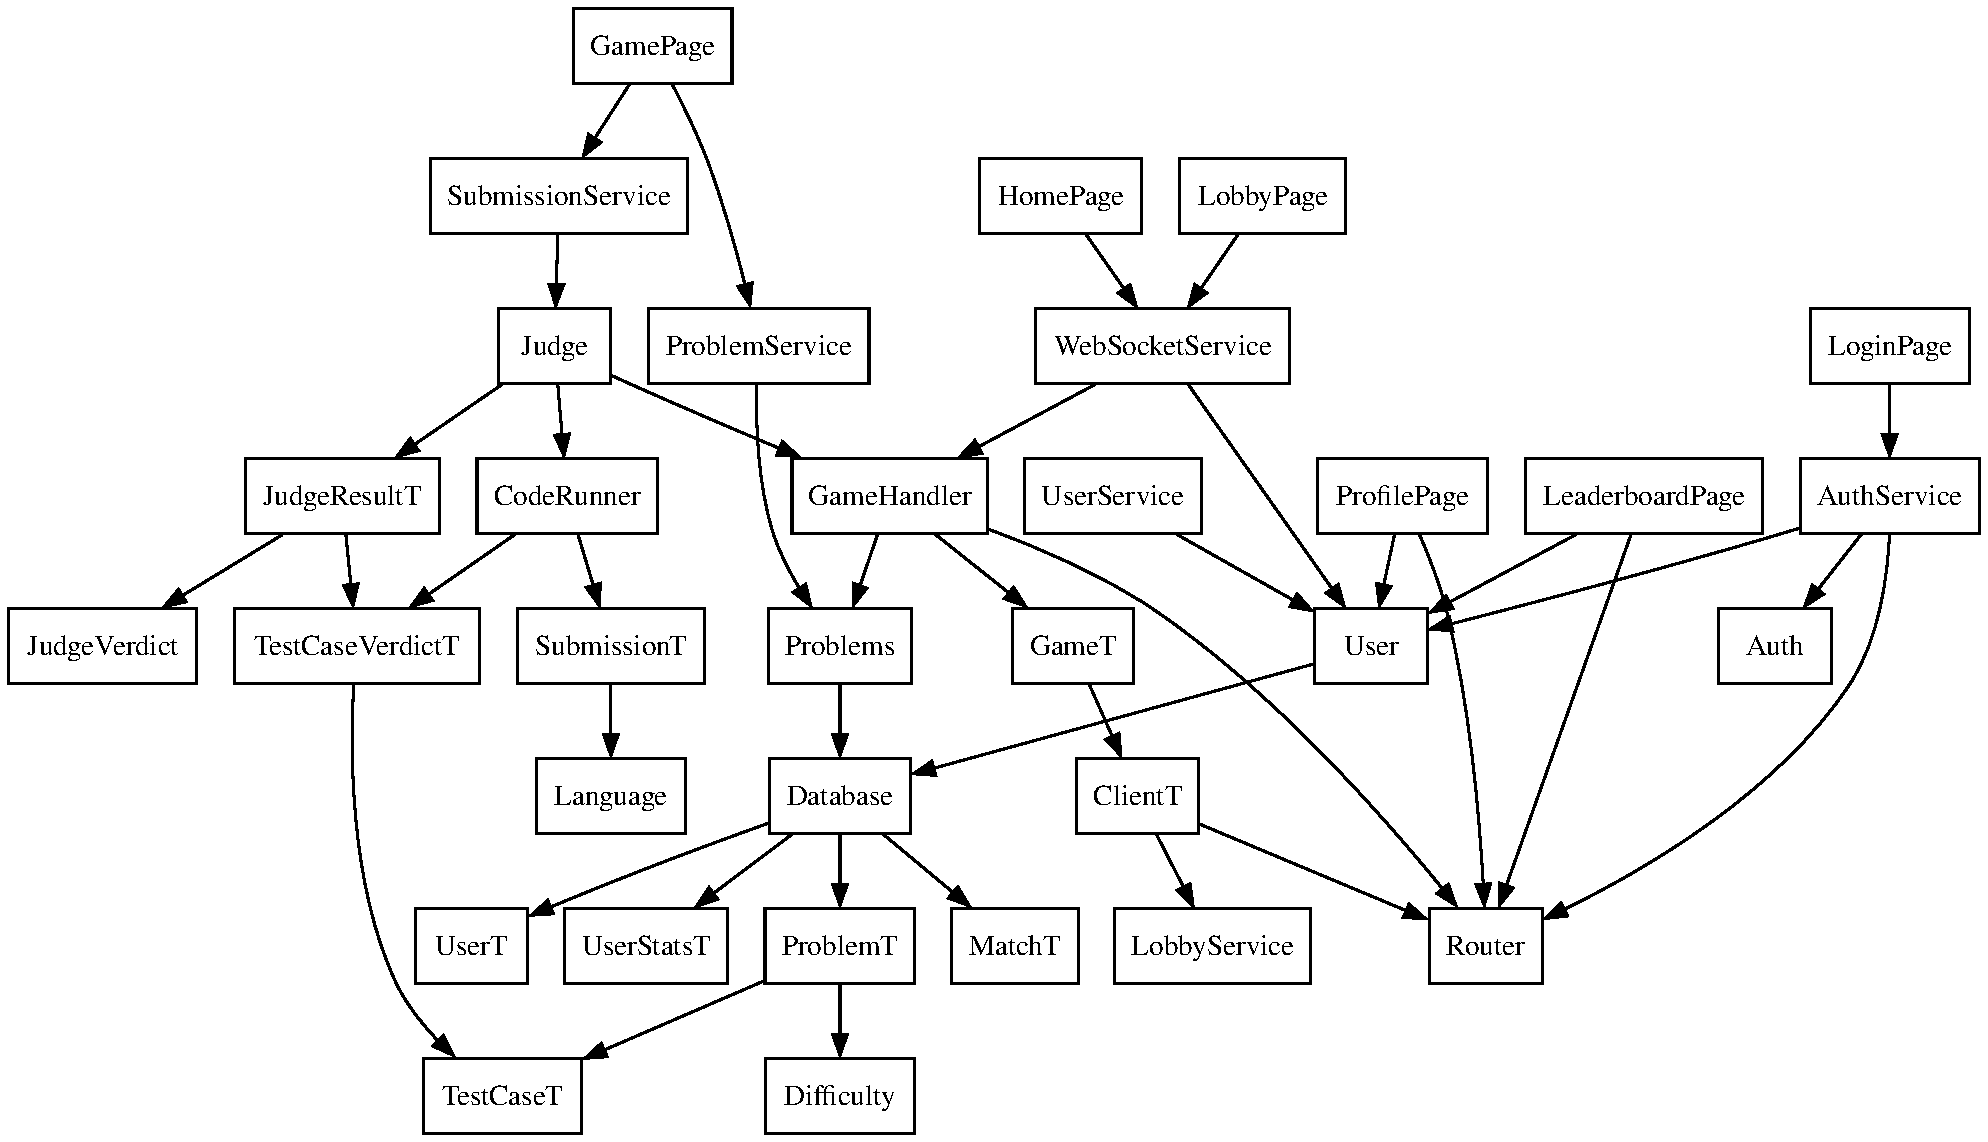
\includegraphics[width=1\textwidth]{UseHierarchy.pdf}
\caption{Use hierarchy among modules}

\label{FigUH}
\end{figure}

%\section*{References}

\bibliographystyle {plainnat}
\bibliography {../../../refs/References}

\newpage{}

\end{document}
